% !TeX program = pdflatex
\documentclass[tikz,border=8pt]{standalone}
\usepackage{tikz}
\definecolor{FigureBlue}{HTML}{2563EB}\definecolor{FigureOrange}{HTML}{EA580C}
\begin{document}
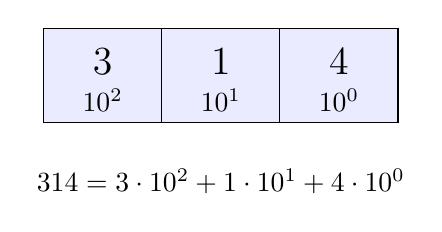
\begin{tikzpicture}
  \foreach \x/\digit/\power in {0/3/$10^2$,1/1/$10^1$,2/4/$10^0$}{\draw[fill=blue!8] (1.5*\x,0) rectangle ++(1.5,1.2);\node at (1.5*\x+.75,.78) {\Large\digit};\node at (1.5*\x+.75,.28) {\power};}
  \node at (2.25,-.75) {$314=3\cdot10^2+1\cdot10^1+4\cdot10^0$};
\end{tikzpicture}
\end{document}
